\section{ラベルの設計}
\label{sec_label}
ボケに付与するラベルは，最初から決まっていたわけではなく，実例の読解，試験的な分類，自動判定の結果を踏まえて段階的に改訂した．
本章では，その経緯と最終の定義を述べる．

\subsection{実例の読解と試験的な分類}
最初に，ボケのラベルとして「画像中のオブジェクトの知識に基づくか否か」「カルタの制約」「お題文への応答」「画像中の文字に基づくか」の4つの観点を候補とした．
これらが実際のボケに適用できるかを確かめるため，お題のラベルで7つの層を作り，層ごとに4件のお題を抽出した．
7つの層は，カルタ，穴埋め，お題文，通常の写真で文字を含むもの，通常の写真で文字を含まないもの，アニメまたは漫画を含むもの，それ以外の媒体である．
各お題から評価の上位3件と無作為の2件のボケを取り，計140件のボケをお題画像と並べて読んだ．
図\ref{fig_pilot}に一覧の例を示す．

\begin{figure}[t]
    \centering
    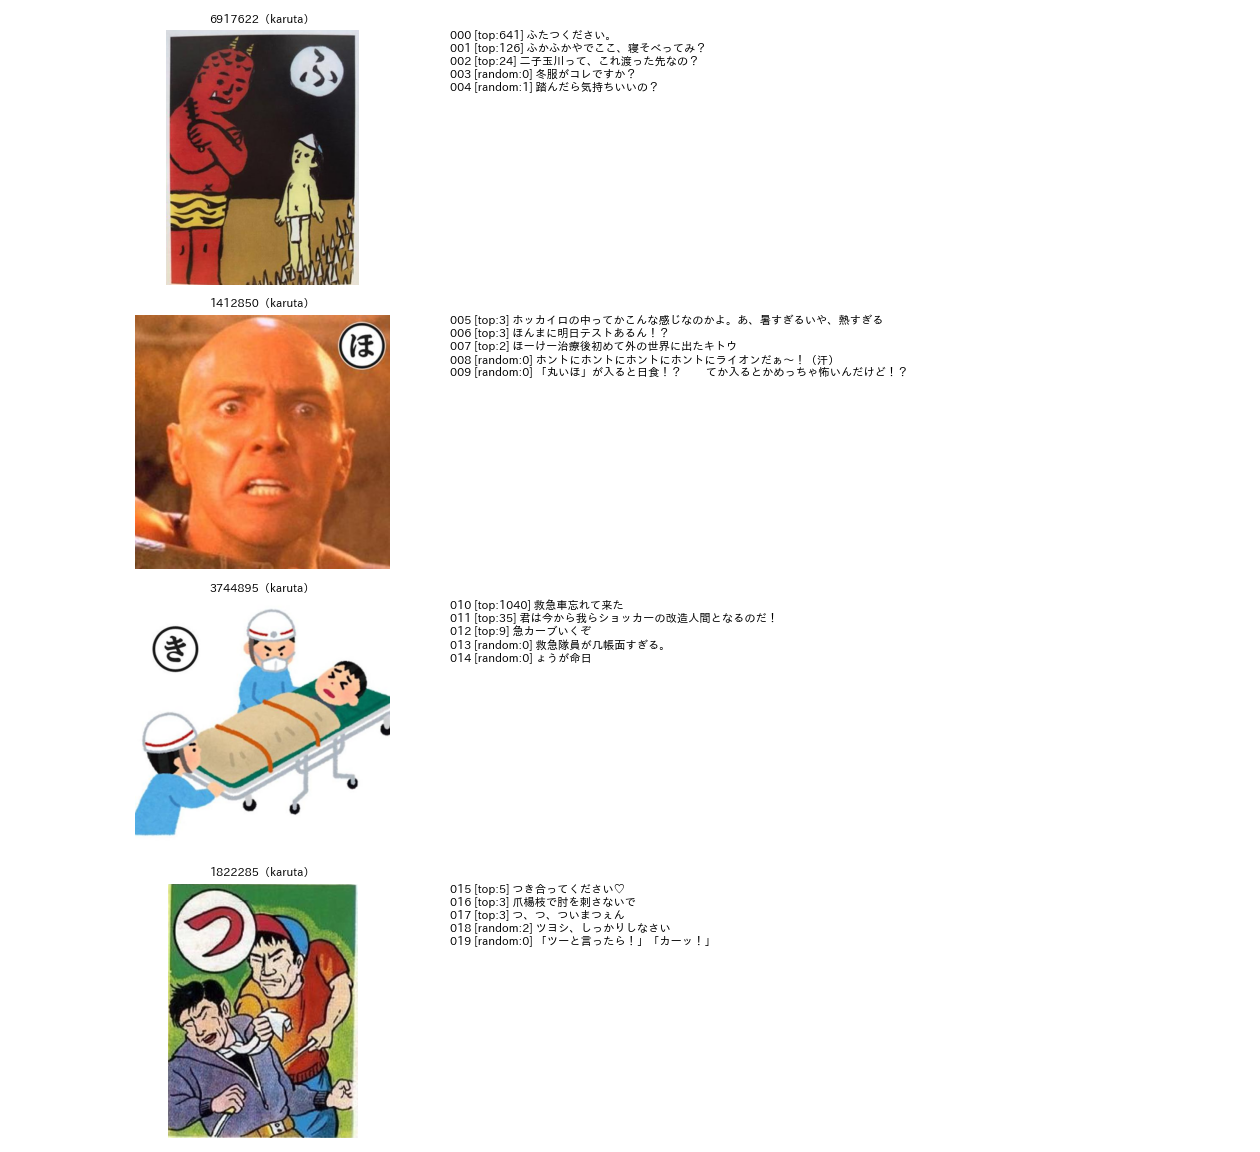
\includegraphics[width=\linewidth]{figures/fig_pilot_sheet.png}
    \caption{実例の読解に用いた一覧の例（カルタのお題）．左がお題画像，右がボケであり，top は評価の上位，random は無作為に選んだボケ，括弧内は評価の合計である．}
    \label{fig_pilot}
\end{figure}

読解の結果，候補の観点は性質の異なる2種類に分かれることが分かった．
一つは，お題の形式が課す制約である．
カルタの札のかなから始めることや，お題文の問いに答えることは，お題の形式でほぼ決まり，ボケに付けるべきなのは「制約に従っているか」だけである．
実際，かなで始まるボケが5件以上あるカルタのお題217件では，最も多い書き出しのかなの割合の中央値が0.91であり，制約はよく守られていた．
もう一つは，ボケの内容に関わる観点であり，こちらがボケ自体に付けるべき主なラベルである．

内容に関わる観点は，「知識に基づくか否か」の1軸では足りなかった．
140件に試験的に分類を付けたところ，知識の要らないボケは26\%にとどまり，一般常識が31\%，画像に写っていない番組・歌・CM・地域などの知識が31\%，画像に写る特定の人物やキャラクターの同定が11\%であった．
画像に写る対象の知識と，画像の外の文化や時事の知識では，生成でも判定でも必要な処理が異なるため，分けて扱う必要がある．
また，ボケは「誰の視点の，どのような言葉か」によって，セリフ，心の声，ツッコミ，状況の説明，名付け・見立て，回答に分かれた．
例えば，卓球選手が大きく反った写真には，「「起立」「気を付け」「ちょ礼」」のように画像の人物の掛け合いを書くボケと，「セルフ膝カックン！！！」のように画像に名前を付けるボケがあった．
以下では，この区分を発話の型と呼ぶ．
表\ref{tab_voice_examples}に，試験的な分類で見られた発話の型の例を，表\ref{tab_know_examples}に必要な知識の例を示す．

\begin{table}[t]
    \centering
    \caption{発話の型の例（試験的な分類より）．}
    \label{tab_voice_examples}
    \footnotesize
    \begin{tabular}{@{}p{0.27\linewidth}p{0.66\linewidth}@{}}
        \toprule
        型 & ボケの例 \\
        \midrule
        セリフ（S） & 「署長、こいつ下は隠さないのに顔は隠すんです。」 \\
        心の声（M） & 「男「どの秘密がバレたんだろう・・・」」 \\
        ツッコミ（T） & 「救急隊員が几帳面すぎる。」 \\
        状況の説明（N） & 「自宅でよさこいの練習をしていたらタンスの角に小指をぶつけた」 \\
        名付け・見立て（L） & 「異常な反応をしたリトマス紙」，「パステルのなめらかプリンを初めて食った時の俺」 \\
        回答（A） & 「サザエさん最終回のタイトルとは？」に「サザエンド」 \\
        \bottomrule
    \end{tabular}
\end{table}

\begin{table}[t]
    \centering
    \caption{必要な知識の4段階の例（試験的な分類より）．}
    \label{tab_know_examples}
    \footnotesize
    \begin{tabular}{@{}p{0.27\linewidth}p{0.66\linewidth}@{}}
        \toprule
        段階 & お題とボケの例 \\
        \midrule
        見た目だけ（0） & 赤ちゃんを抱いて寝る男性に「さ〜て。夜泣き開始。」 \\
        一般常識（G） & 「一石二鳥」の例えに「トイレ行ったら両方出た。」 \\
        画像中の対象（I） & ドラえもんのしずかちゃんのバイオリンに「バイオリン界のジャイアン」 \\
        画像外の事物（O） & チンパンジーの写真に「池の水抜いたらチンパンジー出てきた」（テレビ番組） \\
        \bottomrule
    \end{tabular}
\end{table}

\subsection{定義書の改訂}
試験的な分類を基に定義書を作成し，自動判定の結果と目視ラベルの見直しを踏まえて3回改訂した．
表\ref{tab_versions}に改訂の経緯を示す．

\begin{table}[t]
    \centering
    \caption{定義書の改訂の経緯．}
    \label{tab_versions}
    \small
    \begin{tabular}{@{}p{0.11\linewidth}p{0.47\linewidth}p{0.32\linewidth}@{}}
        \toprule
        版 & 主な内容 & 改訂の根拠 \\
        \midrule
        第1版 & 制約の順守，発話の型6区分，必要な知識4段階，画像中の文字への依存，性的・不適切の5項目 & 試験的な分類（140件） \\
        第2版 & 性的・不適切を削除．必要な知識を上から順に判定する手順とした & 不適切の自動判定が全ての方法で再現率0.27以下 \\
        第3版 & 必要な知識を画像外の知識の2値とし，条件と手順を厳密に定義．発話の型を判定の手順として定義し，3区分を併記 & 4段階の自動判定のマクロ F1 が0.48以下 \\
        \bottomrule
    \end{tabular}
\end{table}

第1版では，必要な知識を，見た目だけで分かる（0），一般常識（G），画像中のオブジェクトの情報（I），画像外のオブジェクト・事象の情報（O）の4段階とした．
当初は「画像に写る対象の同定」と呼んでいたが，固有名詞を言い当てられるかはモデルに依存するため，名前を言えるかではなく必要な情報の種類で判断するよう改めた．
また，お題文の「サザエさん」のように画像中の文字で名指しされた対象は，画像中のオブジェクトとした．

性的・不適切の項目は，検証データ（\ref{sec_validation}章）の6.4\%が該当したが，VLM の教師は性的なほのめかしの多くを見落とし，教師ラベルでの陽性率は0.9\%にとどまった．
その結果，教師ラベルで学習した分類器は陽性を1件も予測せず，最良の方法でも F1 0.42，再現率0.27にとどまった．
この項目は専用のデータを作らなければ扱えないと判断し，第2版で削除した．

必要な知識の4段階は，目視では上から順に判定すれば迷いが少なかった．
しかし，\ref{sec_text}章で述べるとおり，自動判定では4段階のマクロ F1 が最高でも0.48であり，見た目だけと一般常識の混同と，画像中と画像外の区別の難しさが残った．
一方，画像外の知識が要るか否かの2値は比較的安定して判定できた．
下流の生成や判定でも，外部の知識が要るボケを分けることが最も重要であるため，第3版では2値に改めた．

\subsection{最終の定義}
第3版の定義書は，次の4項目からなる．

\textbf{制約の順守}は，お題の形式が課す制約にボケが従っているかであり，はい，いいえ，対象外（通常の形式）の3値とする．
カルタは書き出しが札のかなと同じ音で始まるか，穴埋めは空欄に入る語句であるか，お題文は問いや指示に応じているかで判断する．
お題と無関係な書き込みは，形式によらず「いいえ」とする．

\textbf{発話の型}は，ボケが誰の視点の，どのような言葉であるかである．
6区分は，次の問いを順に確かめて決める．
\begin{enumerate}
    \item 形式が穴埋め・お題文で，ボケが空欄や問いへの答えであれば，回答（A）とする．
    \item ボケが名詞句で，画像全体や写っている物に名前・題・例えを付けていれば，名付け・見立て（L）とする．
    \item 話し手が画像の中の人物・動物・物であれば，声に出している言葉をセリフ（S），心の中の考えや独り言を心の声（M）とする．迷う場合はセリフとする．
    \item 話し手が画像の外の人であれば，画像の出来事や前後の状況を説明する文を状況の説明（N），画像を見て言う感想・指摘・ツッコミや画像の人物への呼びかけをツッコミ（T）とする．
\end{enumerate}
6区分は人でも判断が分かれやすいため，信頼性の低いラベルとして扱い，登場人物の言葉（S，M），外からの言葉（T，N，L），回答（A）の3区分を併記する．

\textbf{画像外の知識}は，面白さを理解するのに，画像にも画像中の文字にも示されていない特定の事物の知識が必要かであり，次の3条件を全て満たすときに「はい」とする．
\begin{enumerate}
    \item 特定性：依存する事物が，特定の作品・人物・商品・番組・歌・地名の印象・出来事・流行語・ネットの定型・有名な台詞・ボケての慣習などである．
    \item 画像の外：その事物が画像に写っておらず，画像中の文字でも名指しされていない．
    \item 必要性：その事物を知らないと面白さが成り立たない．
\end{enumerate}
一般の語彙，慣用句，ラジオ体操のように誰もが知る生活の事物，一般的な職業やジャンルの印象は「いいえ」とする．

\textbf{画像中の文字への依存}は，ボケの意味が画像中の文字を読まないと分からないかである．
この項目は形式でほぼ決まり，穴埋め・お題文は依存し，通常はほぼ依存しない．
第1版の検証データ（最終評価用210件）で，形式だけの規則で F1 0.77，\ref{sec_text}章で述べる目視ラベルによる補正で F1 0.90 が得られたため，以下では詳しく扱わない．
